\newpage

\section{Simulation Analysis}
\label{sec:simulation}

\subsection{Simple circuit}

\begin{figure}[H]
\centering
\includegraphics[width=0.6\textwidth]{gain_sim}
\caption{Data collected versus simulated data}
\label{data_graph_sim}
\end{figure}

It is obvious, from the above graph, that there are slight deviations between the real data and the simulated data, as expected. This can be due to any number of experimental causes:

\begin{itemize}

\item Errors in the peak to peak amplitude determined by the oscilloscope

\item Errors in the resistors used in the lab (had gold tolerance)

\item Errors in the capacitors used in the lab

\item For the $500\;\Omega$ resistor, two $1\;k\Omega$ resistors were employed, in parallel

\item All signals went through the breadboard

\item $V_{CC}$ was not exactly $10\;V$ and $V_{EE}$ was not exactly $-10\;V$

\item Discrepancies in the {\bf Ngpisce} models

\end{itemize}

Using the same parameters of the laboratory, the following was obtained:

\begin{table}[H]
  \centering
  \begin{tabular}{|c|c|}
    \hline
        {\bf Name} & {\bf Value} \\
        \hline
        \hline
        \input{lab}
        \hline
  \end{tabular}
  \caption{Simulation results}
  \label{sim_results}
\end{table}

\begin{figure}[H]
\centering
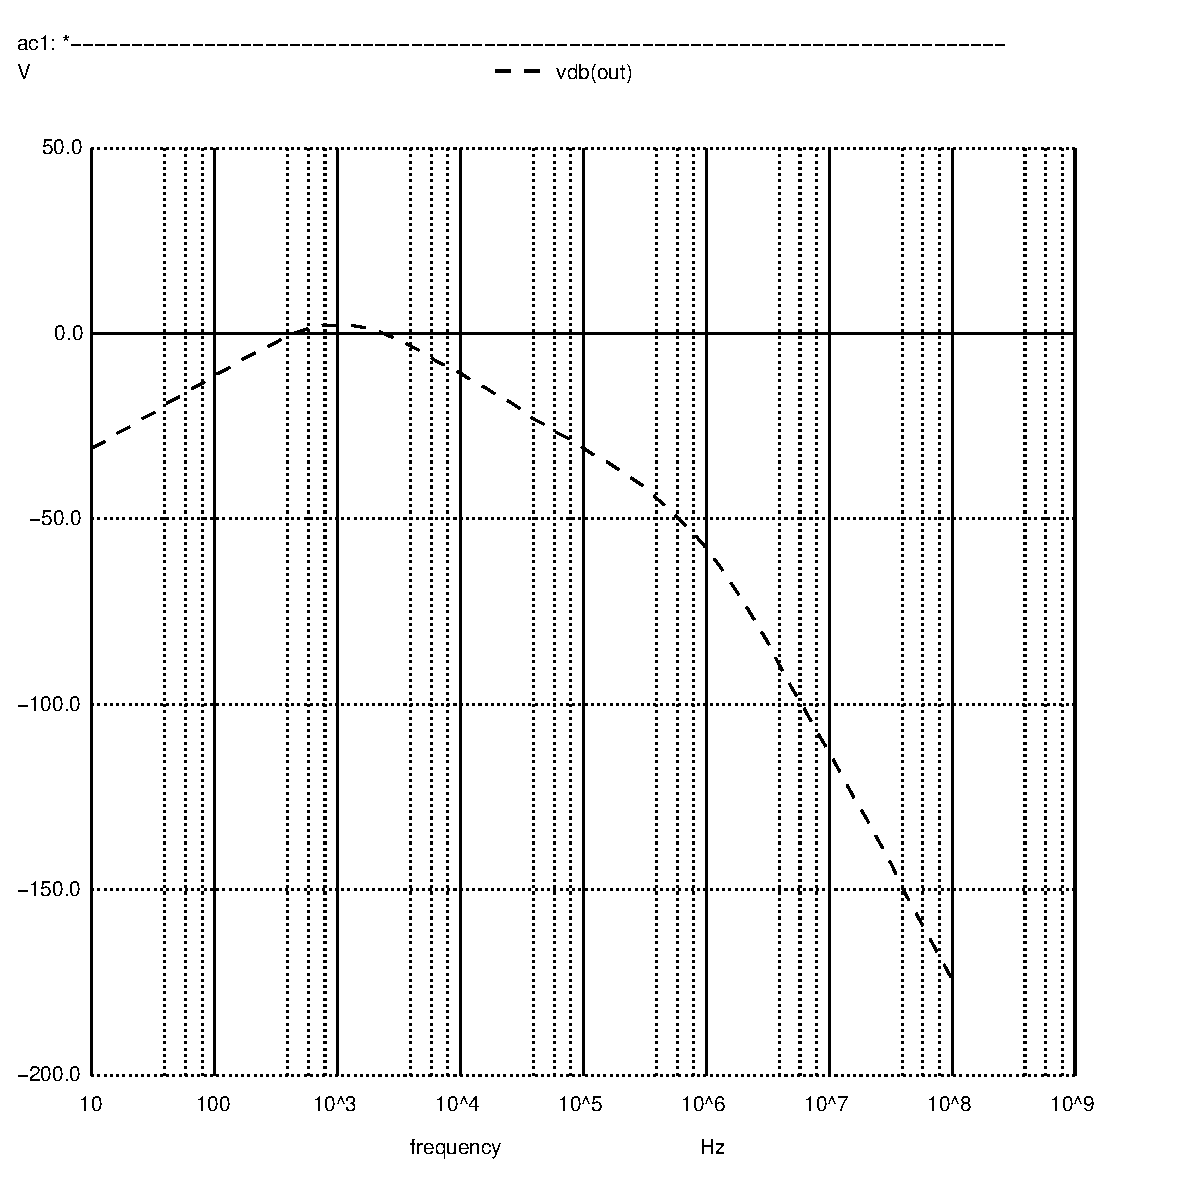
\includegraphics[width=0.6\textwidth]{vo1f}
\caption{Frequency response - Gain}
\end{figure}

\begin{figure}[H]
\centering
\includegraphics[width=0.6\textwidth]{vo1f_phase}
\caption{Frequency response - Phase}
\end{figure}

\newpage

\subsection{Optimized circuit}

By a lengthy process of trial and error, attempting to maximize the merit figure, while using only the components available, the following parameters were obtained:

\begin{table}[H]
\centering
\begin{tabular}{|c|c|}
        \hline
        Parameter & Value \\
        \hline
        $C_1 (nF)$ & 220 \\
        $R_1 (k\Omega)$ & 1 \\
        $C_2 (nF)$ & 110 (two 220 in series) \\
        $R_2 (k\Omega)$ & 1 \\
        $R_4 (k\Omega)$ & 1 \\
        $R_5 (k\Omega)$ & 105 (one 100 in series with two 10 in parallel) \\
        \hline
\end{tabular}
\caption{Parameters for the optimized circuit}
\label{optimized_par}
\end{table}

\begin{table}[H]
  \centering
  \begin{tabular}{|c|c|}
    \hline
        {\bf Name} & {\bf Value} \\
        \hline
        \hline
        $f_c\; (Hz)$ & 262.77028969352676 \\ 
 \hline 
$gain(f_c)\; (dB)$ & 38.19408 \\ 
 \hline 
$z_{in}$ & 0.4999899 + i ( -0.159204 ) \\ 
 \hline 
$z_{out}$ & 0.341692 + i ( -0.233043 ) \\ 
 \hline 

        \hline
  \end{tabular}
  \caption{Results}
  \label{sim_mb_results}
\end{table}

\begin{figure}[H]
\centering
\includegraphics[width=0.6\textwidth]{vo1f_mb}
\caption{Frequency response - Gain}
\end{figure}

\begin{figure}[H]
\centering
\includegraphics[width=0.6\textwidth]{vo1f_mb_phase}
\caption{Frequency response - Phase}
\end{figure}
